\documentclass[14pt]{beamer}

% font
\usepackage{fontspec}
\setmainfont[Ligatures=TeX]{IPAPGothic}
\usepackage{xeCJK}
\setCJKmainfont{IPAPGothic}
\newfontfamily{\liberation}{Liberation Sans}
\newfontfamily{\notosans}{Noto Sans CJK JP}

% graphic
\usepackage{graphics}
\usepackage{graphicx}
\usepackage{color}
\usepackage{xcolor}
\usepackage{colortbl}
\usepackage{tcolorbox}
\definecolor{mygray}{rgb}{0.1, 0.1, 0.1}

% tikz
\usepackage{tikz}
\usetikzlibrary{automata}
\usetikzlibrary{arrows}
\usetikzlibrary{arrows.meta}
\usetikzlibrary{positioning}
\usetikzlibrary{intersections, calc}
\usetikzlibrary{decorations}
\usetikzlibrary{decorations.markings}
\usetikzlibrary{decorations.pathreplacing,angles,quotes}
\usetikzlibrary{fit}
\usetikzlibrary{math}
\usetikzlibrary{shapes}
\usepackage{pgfplots}
\usepackage{bchart}

% href
\usepackage{hyperref}
\hypersetup{
	colorlinks=true,
	linkcolor=cyan,
	filecolor=cyan,
	urlcolor=cyan,
	pdfnewwindow=true}

% beamer
\usepackage{bxdpx-beamer}
\usetheme{Boadilla}
\setbeamertemplate{navigation symbols}{}
\setbeamercovered{transparent}
\setbeamertemplate{frametitle}{%
	\vspace{0.1em}
	\usebeamerfont{frametitle}\insertframetitle%
	\par
	\rule[0.5\baselineskip]{0.9\paperwidth}{0.4pt}%
	\vspace{-0.5em}}
\setbeamertemplate{footline}{
	\hfill
	\usebeamercolor[fg]{page number in head/foot}
	\usebeamerfont{page number in head/foot}
	{\small \insertframenumber}
	\kern1em\vskip5pt
}
\setbeamercolor{footline}{fg=black,bg=black}

% itemize
\usepackage{enumitem}
\setitemize{itemsep=0.3em}
\setlength\leftmargini{20pt}
\setlength\leftmarginii{20pt}
\setlength\leftmarginiii{20pt}
\setlength\leftmarginiv{20pt}
\setlist[itemize,1]{label=$\color{blue}\bullet$}
\setlist[itemize,2]{label=$\color{orange}\triangleright$}
\setlist[itemize,3]{label=$\color{gray}\bullet$}
\setlist[itemize,4]{label=$\color{red}\triangleright$}
\setlist[itemize,5]{label=$\color{gray}\bullet$}
\setlist[itemize,6]{label=$\color{red}\triangleright$}
\setlist[itemize,7]{label=$\color{yellow}\bullet$}
\setlist[itemize,8]{label=$\color{pink}\triangleright$}
\setlist[itemize,9]{label=$\color{black}\bullet$}

% math
\usepackage{amsmath,amssymb,amsthm}
\usepackage{bm}
\setbeamertemplate{theorems}[numbered]
\theoremstyle{definition}
\newtheorem{thm}{定理}
\newtheorem{lem}{補題}
\newtheorem{prop}{命題}
\newtheorem{dfn}{定義}
\setbeamertemplate{theorem begin}{{
	\inserttheoremheadfont
	\inserttheoremname
	\inserttheoremnumber
	\inserttheorempunctuation
}}
\setbeamertemplate{theorem end}{}

% other
\usepackage{caption}
\usepackage{cancel}
\usepackage{epigraph}
\usepackage{fancybox}
\usepackage{here}
\usepackage{makecell}
\usepackage{setspace}
\usepackage{scrextend}
\usepackage{svg}
\usepackage{ulem}
\usepackage{multirow}

\begin{document}

\begin{frame}
	\begin{center}
		{\LARGE \color{cyan} nymwa\kern.0emさんはなぜ\\土下座大田区一周を\\しなければならないのか} \\
		\vspace{1em}
		{\scriptsize 〜トキポナが正則言語ではないことの証明〜}
	\end{center}
\end{frame}


\begin{frame}
	\frametitle{すべてはこのツイートから始まった}

	\begin{figure}[h]
		\centering
		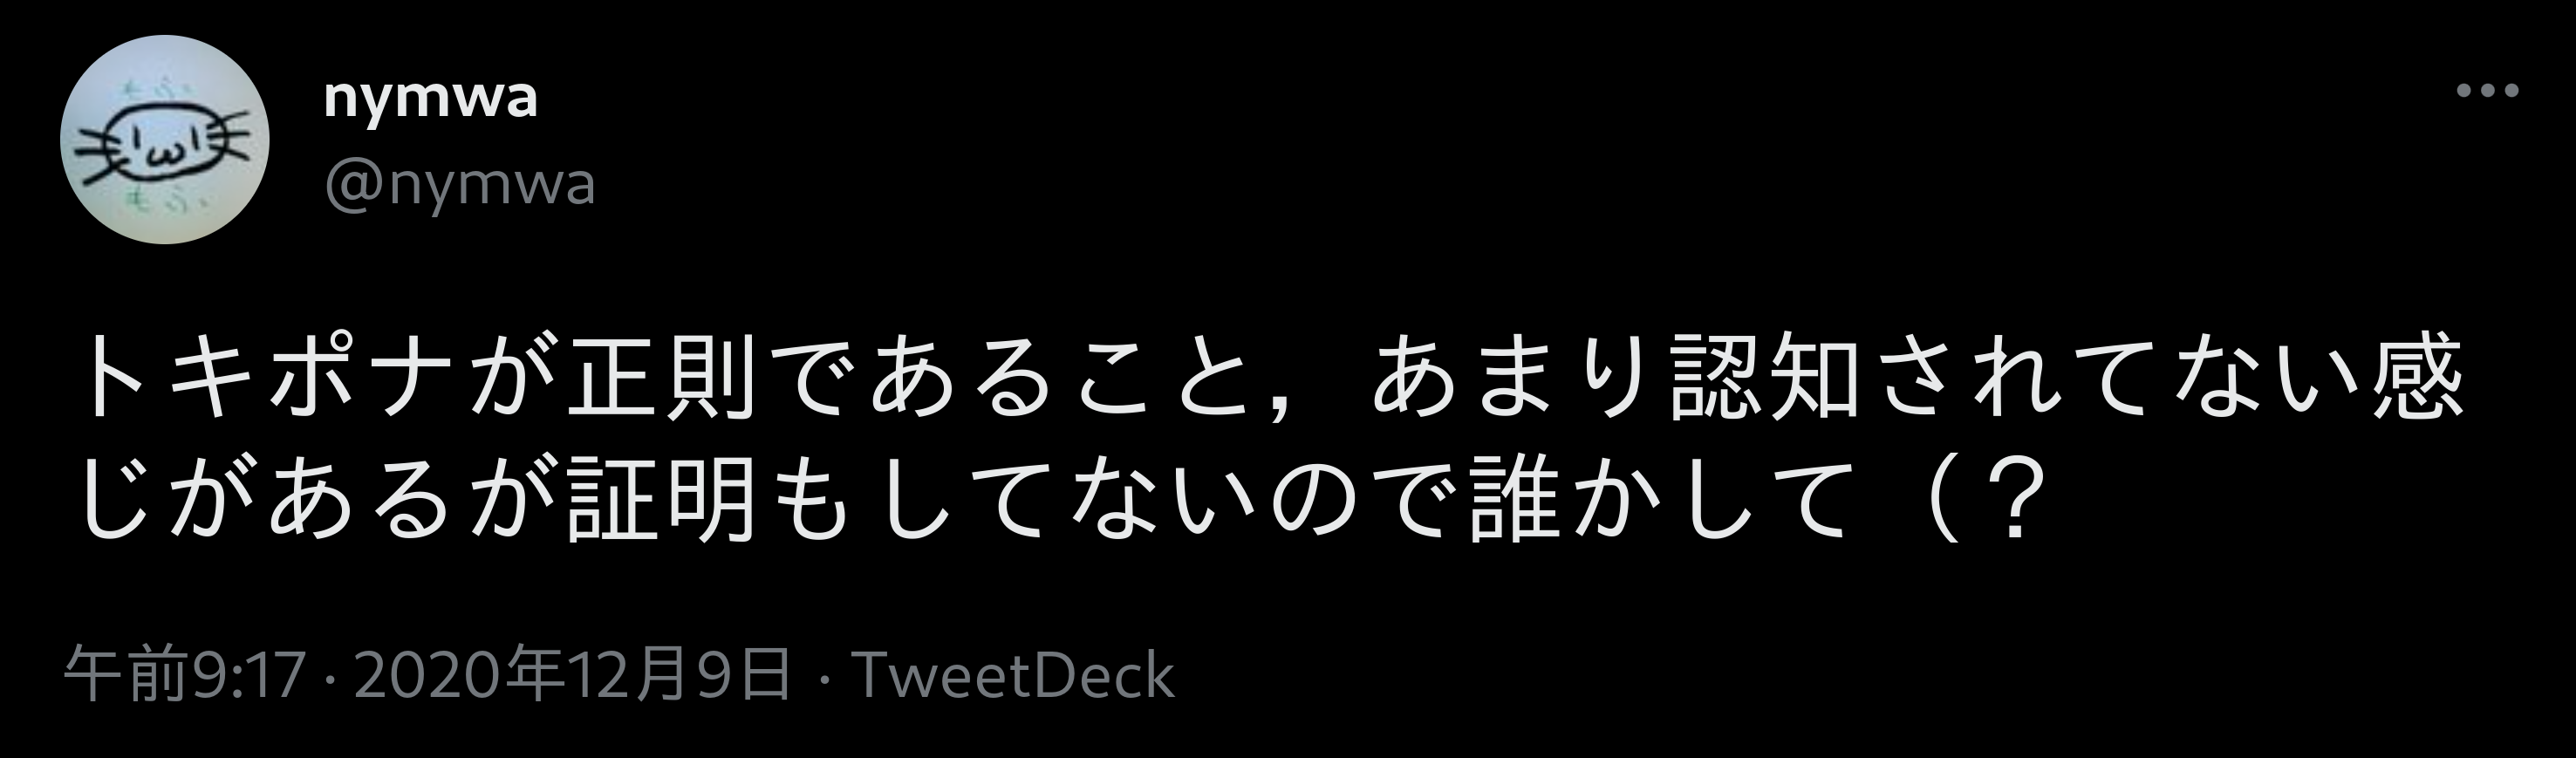
\includegraphics[width=10cm]{tweet1.png}
	\end{figure}

\end{frame}


\begin{frame}
	\frametitle{自らの正しさを信じ切る\kern.0emnymwa}

	\begin{figure}[h]
		\centering
		
\includegraphics[width=10cm]{tweet2.png}
	\end{figure}

\end{frame}


\begin{frame}
	\frametitle{妄言の末路}

	\begin{figure}[h]
		\centering
		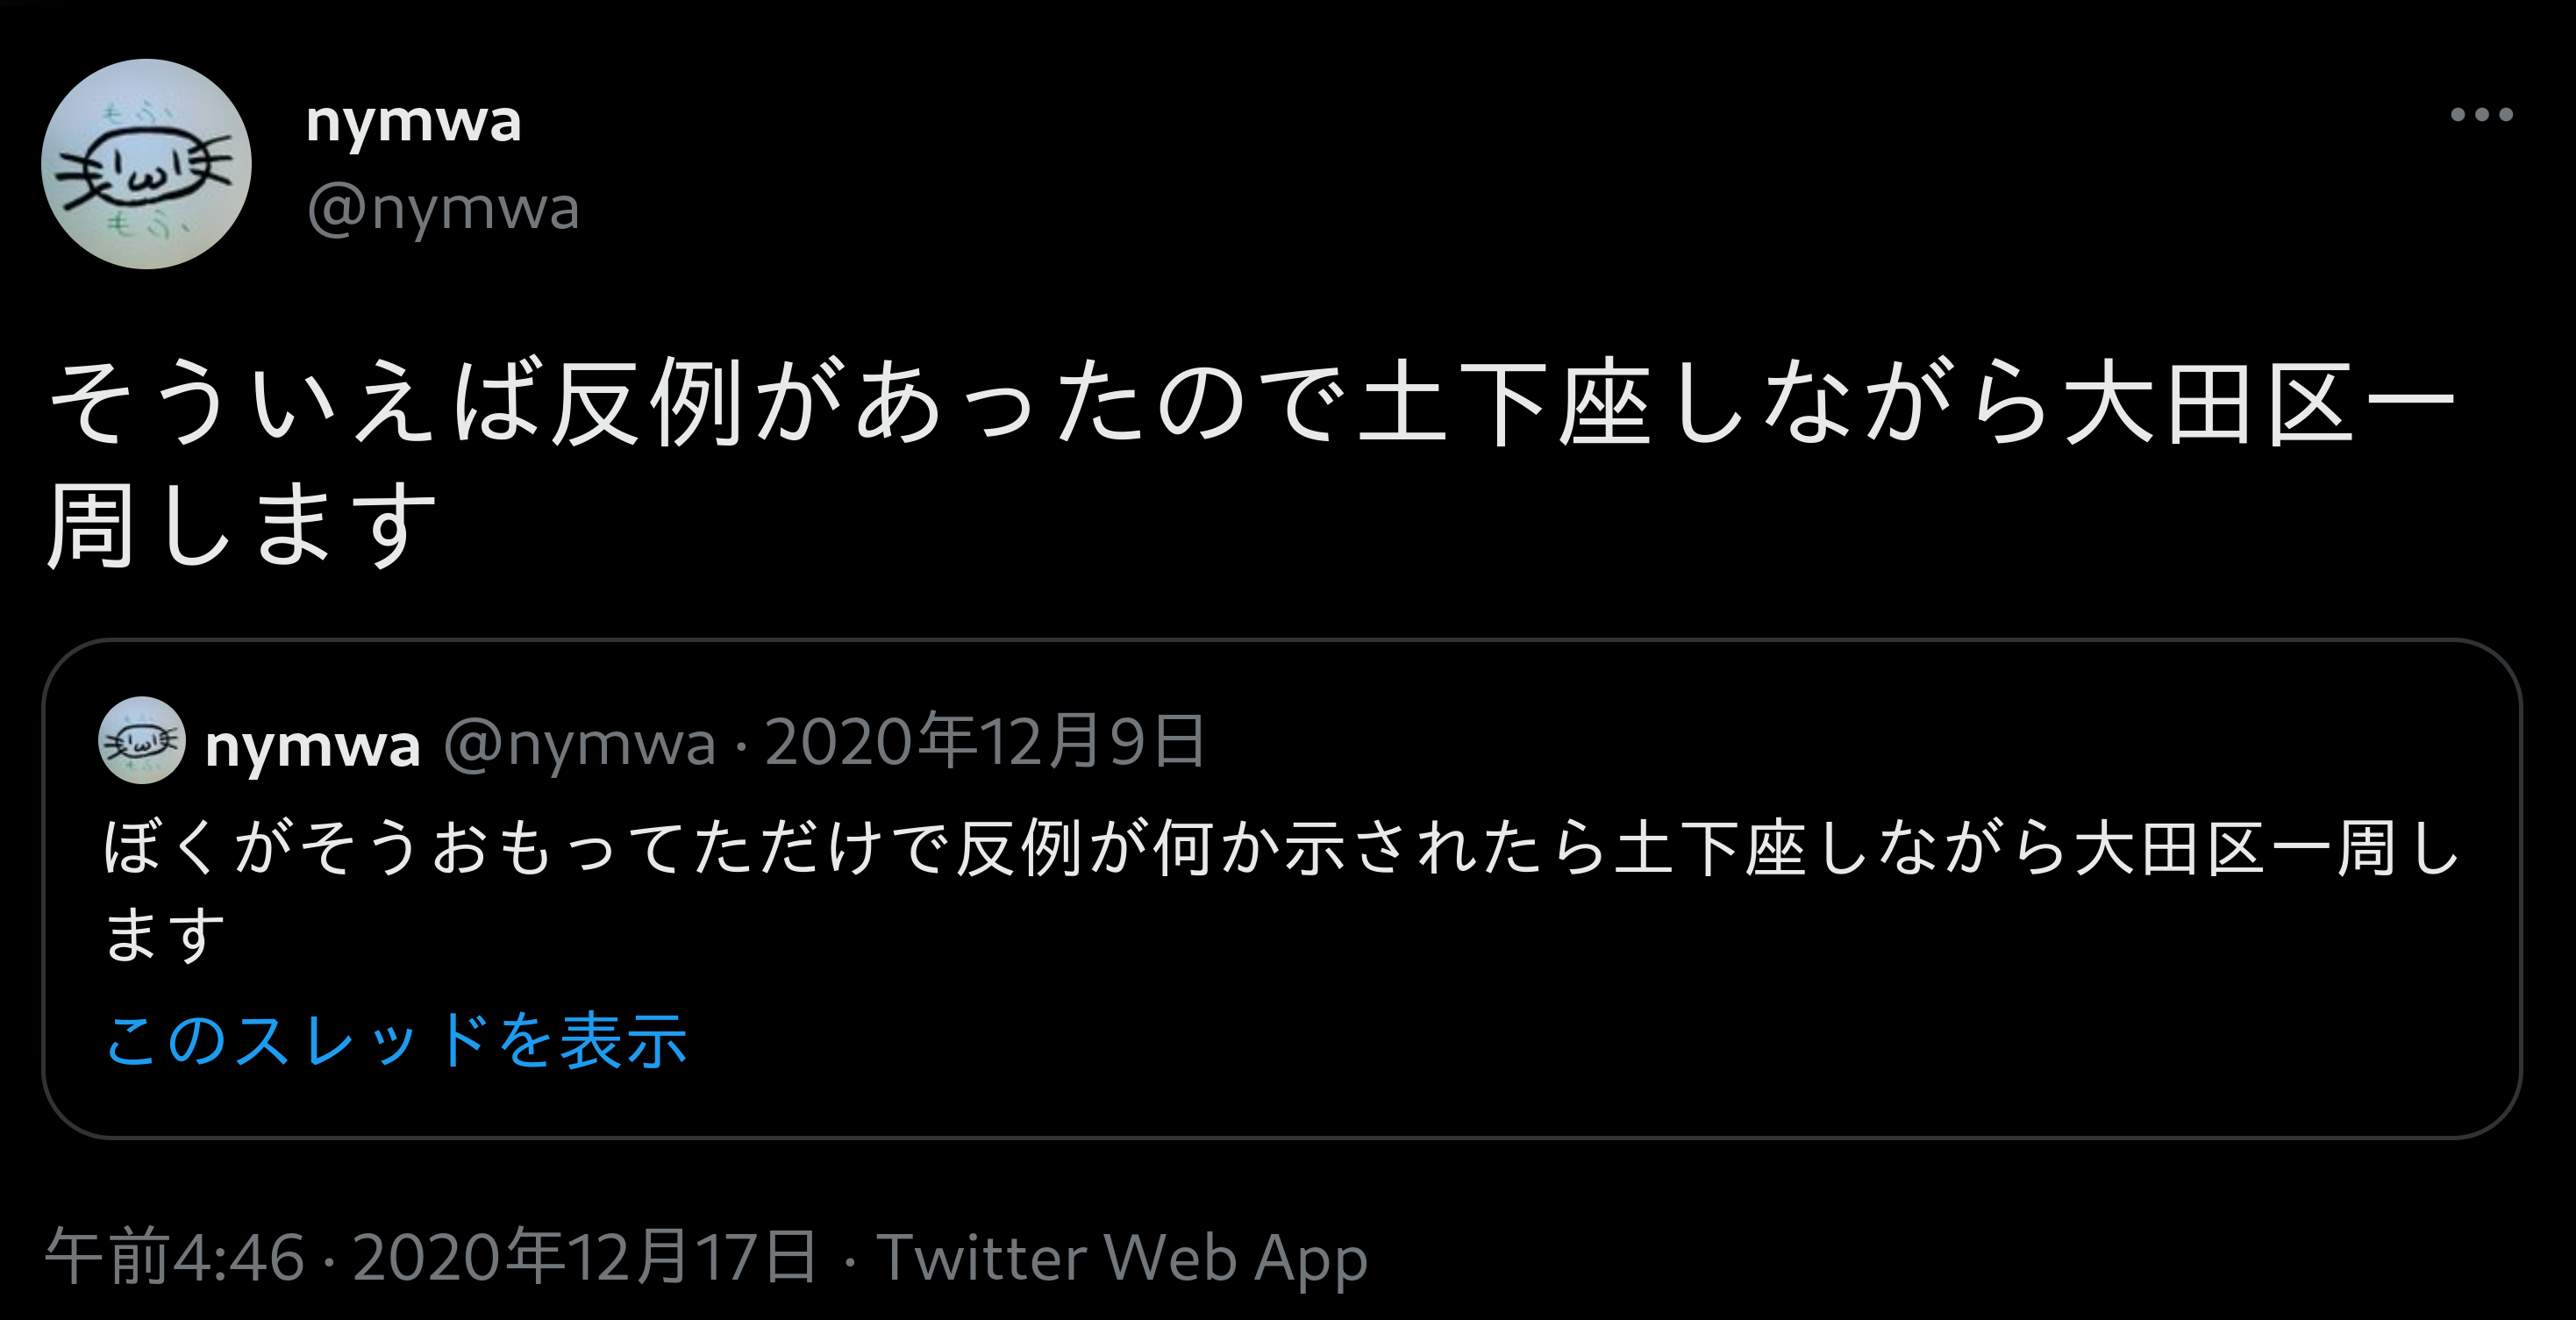
\includegraphics[width=10cm]{tweet3.png}
	\end{figure}

\end{frame}


\begin{frame}
	\frametitle{示したいこと}

	\begin{tcolorbox}[
			colframe=orange!80,
			colback=orange!20,
			sharp corners]
		\begin{prop}\label{prop:pona}
			トキポナは正則言語である.
		\end{prop}

		\begin{thm}
			命題\ref{prop:pona}は偽である.
		\end{thm}
	\end{tcolorbox}

\end{frame}


\begin{frame}
	\frametitle{概要}

	\begin{itemize}
		\item 次のような流れです
			\begin{itemize}
				\item 正則言語・文脈自由言語・文脈依存言語とは?
				\item トキポナは文脈依存言語である証明
				\item トキポナは正則言語ではない!
					\begin{itemize}
						\item 文脈依存なら正則ではない
					\end{itemize}
			\end{itemize}
		\item 最後に土下座大田区一周の概要を説明します
	\end{itemize}

\end{frame}


\begin{frame}
	\frametitle{証明の流れ}

	\begin{itemize}
		\item コピー言語は文脈自由ではない
		\item コピー言語が文脈自由でないならば反復疑問文がある言語は文脈自由でない
		\item トキポナは反復疑問文があるため文脈自由でない
		\item トキポナは正則言語ではない
	\end{itemize}

\end{frame}


\begin{frame}
	\frametitle{形式言語}
\end{frame}


\begin{frame}
	\frametitle{チョムスキー階層}
\end{frame}


\begin{frame}
	\frametitle{正則言語}
\end{frame}


\begin{frame}
	\frametitle{文脈自由言語}
\end{frame}


\begin{frame}
	\frametitle{文脈依存言語}
\end{frame}


\begin{frame}
	\frametitle{なぜトキポナが正則と思ったのか?}

	\begin{itemize}
		\item トキポナはかんたん
			\begin{itemize}
				\item 再帰がない!
					\begin{itemize}
						\item I read the book I bought.
						\item mi esun e lipu. mi lukin e ona.
					\end{itemize}
			\end{itemize}
		\item 再帰がある $\Rightarrow$ 正則ではない
			\begin{itemize}
				\item 文脈自由文法は再帰を記述できる
			\end{itemize}
		\item 「トキポナは再帰がないから正則なのでは?」
			\begin{itemize}
				\item {\color{gray} \small「再帰がない $\to$ 正則である」は真でない…}
			\end{itemize}
	\end{itemize}

\end{frame}


\begin{frame}
	\frametitle{コピー言語}
\end{frame}


\begin{frame}
	\frametitle{コピー言語は文脈自由でない}
\end{frame}


\begin{frame}
	\frametitle{コピー言語は文脈依存}
\end{frame}


\begin{frame}
	\frametitle{反復疑問は文脈依存}
\end{frame}


\begin{frame}
	\frametitle{トキポナは文脈依存}
\end{frame}


\begin{frame}
	\frametitle{トキポナは弱文脈依存文法}
\end{frame}


\begin{frame}
	\frametitle{トキポナは正則でないため…}
\end{frame}


\begin{frame}
	\frametitle{土下座大田区一周の概要}

	\begin{itemize}
		\item 多摩川 - 羽田 区間
			\begin{itemize}
				\item ゴムボートで土下座川下り
			\end{itemize}
		\item 天空橋 - 天王洲アイル 区間
			\begin{itemize}
				\item 土下座モノレール
			\end{itemize}
		\item 品川 - 目黒 区間
			\begin{itemize}
				\item 土下座山手線
			\end{itemize}
		\item 目黒 - 多摩川 区間
			\begin{itemize}
				\item 土下座目黒線
			\end{itemize}
		\item 乗り換えで歩くのは許してほしい
	\end{itemize}

\end{frame}

\end{document}

